\PassOptionsToPackage{subsection=false}{beamerouterthememiniframes}
\PassOptionsToPackage{dvipsnames,table}{xcolor}
\documentclass[fleqn]{beamer}
\usepackage{graphicx}
\usepackage{multirow}
\usepackage{multicol}
\usepackage{amsmath,amsfonts,amsthm,amsopn}
\usepackage{color, colortbl}
\usepackage{subfig}
\usepackage{wrapfig}
\usepackage{fancybox}
\usepackage{tikz}
\usepackage{fancyhdr}
\usepackage{setspace}
\usepackage{xcolor}
\usepackage{movie15}
\usepackage{pifont}
\usepackage{soul}
\usepackage{fancyvrb,newverbs}
\usepackage{epsfig}
\usepackage{epstopdf}
\fvset{fontsize=\footnotesize}
\RecustomVerbatimEnvironment{verbatim}{Verbatim}{}

%\usepackage{fancybox}

\usetheme{Szeged}
\usecolortheme{default}

%\definecolor{links}{HTML}{2A1B81}
%\definecolor{links}{blue!20}
\hypersetup{colorlinks,linkcolor=,urlcolor=blue!80}

\setbeamertemplate{blocks}[rounded]
\setbeamercolor{block title}{bg=blue!40,fg=black}
\setbeamercolor{block body}{bg=blue!10}


\newenvironment<>{clicker}[1]{%
  \begin{actionenv}#2%
      \def\insertblocktitle{#1}%
      \par%
      \mode<presentation>{%
        \setbeamercolor{block title}{fg=white,bg=magenta}
       \setbeamercolor{block body}{fg=black,bg=magenta!10}
       \setbeamercolor{itemize item}{fg=magenta}
       \setbeamertemplate{itemize item}[triangle]
       \setbeamercolor{enumerate item}{fg=magenta}
     }%
      \usebeamertemplate{block begin}}
    {\par\usebeamertemplate{block end}\end{actionenv}}

%\newcommand{\bmp}{\begin{minipage}}
%\newcommand{\emp}{\end{minipage}}
%\newcommand{\blankcolumn}{\bmp{.05\textwidth}\hspace{0.50in} \emp}

\defbeamertemplate*{footline}{infolines theme}
{
  \leavevmode%
  \hbox{%
  \begin{beamercolorbox}[wd=.333333\paperwidth,ht=2.25ex,dp=1ex,left]{author in head/foot}%
    \usebeamerfont{author in head/foot}~~\insertshortinstitute: \insertshorttitle
  \end{beamercolorbox}%
  \begin{beamercolorbox}[wd=.67\paperwidth,ht=2.25ex,dp=1ex,right]{date in head/foot}%
    \usebeamerfont{date in head/foot}%\insertshortdate{}\hspace*{2em}
    \insertframenumber{} / \inserttotalframenumber\hspace*{2ex}
  \end{beamercolorbox}
  }%
  \vskip0pt%
}

\newcommand{\cmark}{\ding{51}}%
\newcommand{\xmark}{\ding{55}}%
\newcommand{\grp}{\textcolor{magenta}{Group Exercise}}
\newcommand{\grpc}{\textcolor{magenta}{Group Exercise, continued}}
\newcommand{\bsans}[1]{\underline{\hspace{0.2in}\color{blue!80}{#1}\hspace{0.2in}}}

\definecolor{cverbbg}{gray}{0.93}
\newenvironment{cverbatim}
 {\SaveVerbatim{cverb}}
 {\endSaveVerbatim
  \flushleft\fboxrule=0pt\fboxsep=.5em
  \colorbox{cverbbg}{\BUseVerbatim{cverb}}%
  \endflushleft
}
\newenvironment{lcverbatim}
 {\SaveVerbatim{cverb}}
 {\endSaveVerbatim
  \flushleft\fboxrule=0pt\fboxsep=.5em
  \colorbox{cverbbg}{%
    \makebox[\dimexpr\linewidth-2\fboxsep][l]{\BUseVerbatim{cverb}}%
  }
  \endflushleft
}

\newcommand{\bmp}{\begin{minipage}}
\newcommand{\emp}{\end{minipage}}
\newcommand{\blankcolumn}{\bmp{.05\textwidth}\hspace{0.50in} \emp}

 \newenvironment{code}[1]%
  {\vspace{.1in}\footnotesize\Verbatim[frame=single,label=SAS Code,commandchars=\\\{\},xrightmargin=#1\textwidth,framesep=.2in,labelposition=all]}
  {\endVerbatim\normalsize}

 \newenvironment{Rcode}[1]%
  {\vspace{.1in}\footnotesize\Verbatim[frame=single,label=R Code,commandchars=\\\{\},xrightmargin=#1\textwidth,framesep=.2in,labelposition=all]}
  {\endVerbatim\normalsize}

   \newenvironment{RcodeScript}[1]%
  {\vspace{.1in}\scriptsize\Verbatim[frame=single,label=R Code,commandchars=\\\{\},xrightmargin=#1\textwidth,framesep=.2in,labelposition=all]}
  {\endVerbatim\normalsize}

 \newenvironment{RcodeTiny}[1]%
  {\vspace{.1in}\tiny\Verbatim[frame=single,label=R Code,commandchars=\\\{\},xrightmargin=#1\textwidth,framesep=.2in,labelposition=all]}
  {\endVerbatim\normalsize}


   \newenvironment{Rout}[1]%
  {\vspace{.1in}\footnotesize\Verbatim[frame=single,label=R Output,commandchars=\\\{\},xrightmargin=#1\textwidth,framesep=.2in,labelposition=all]}
  {\endVerbatim\normalsize}
  
     \newenvironment{MTout}[1]%
  {\vspace{.1in}\footnotesize\Verbatim[frame=single,label=Minitab Output,commandchars=\\\{\},xrightmargin=#1\textwidth,framesep=.2in,labelposition=all]}
  {\endVerbatim\normalsize}

   \newenvironment{RoutScript}[1]%
  {\vspace{.1in}\scriptsize\Verbatim[frame=single,label=R Output,commandchars=\\\{\},xrightmargin=#1\textwidth,framesep=.2in,labelposition=all]}
  {\endVerbatim\normalsize}

 \newenvironment{RoutTiny}[1]%
  {\vspace{.1in}\tiny\Verbatim[frame=single,label=R Output,commandchars=\\\{\},xrightmargin=#1\textwidth,framesep=.2in,labelposition=all]}
  {\endVerbatim\normalsize}

\newenvironment{craw}[2]%
{\vspace{.1in}\footnotesize\Verbatim[frame=single,label=#2,commandchars=\\\{\},xrightmargin=#1\textwidth,framesep=.2in,labelposition=all]}
  {\endVerbatim\normalsize}


\newenvironment{scriptcraw}[2]%
{\vspace{.1in}\scriptsize \Verbatim[frame=single,label=#2,commandchars=\\\{\},xrightmargin=#1\textwidth,framesep=.2in,labelposition=all]}
  {\endVerbatim\normalsize}

  \newenvironment{tinycraw}[2]%
{\vspace{.1in}\tiny \Verbatim[frame=single,label=#2,commandchars=\\\{\},xrightmargin=#1\textwidth,framesep=.2in,labelposition=all]}
  {\endVerbatim\normalsize}




\title[Set 2]{Functions of $T$}
\author[Pileggi]{Shannon Pileggi}

\institute[STAT 417]{STAT 417}

\date{}


\begin{document}

\begin{frame}
\titlepage
\end{frame}

\begin{frame}
\frametitle{OUTLINE\qquad\qquad\qquad} \tableofcontents[hideallsubsections]
\end{frame}


%===========================================================================================================================
\section[Survival function]{Survival function}
%===========================================================================================================================

\subsection{}

\begin{frame}
\frametitle{The survival function: $S(t)$}
%\item Now that we've discussed particular features of time-to-event data and introduced some notation and terminology, we introduce methods for examining and summarizing the values of the time-to-event variable $T$.

\begin{itemize}
\item[$F(t)$] $\rightarrow$ gives the probability that the time to event is (less than/greater than) time $t$ %less than
\item[] $\rightarrow$ i.e., the probability that an individual  (does/does not) survive \emph{beyond} time $t$ %does not
\item[]
\item[$S(t)$] $\rightarrow$ gives the probability that the time to event is (less than/greater than) time $t$  %greater than
\item[] $\rightarrow$ i.e., the probability that an individual (does/does not) survive \emph{beyond} time $t$ %does
\item[]
\item[$S(t) = $]
%S(t)  = 1 - F(t) = P(T > t) = integral.
\item[]
\item[]
\end{itemize}
\end{frame}



\begin{frame}
\frametitle{Interpretations of $S(t)$}
Two primary interpretations of $S(t)$:
\begin{enumerate}
\item The unconditional probability that a randomly selected individual in the population will survive beyond (not experience the event of interest after) time $t$, and;
\item The proportion of subjects in a population who have yet to experience the event of interest after time $t$.
\item[]
\end{enumerate}
Two \textbf{incorrect} interpretations of $S(t)$:
\begin{enumerate}
\item $S(t)\neq$ the probability that a subject experiences the event after time $t$
\item $S(t)\neq$ the probability that the subject experiences the event at time $t$
\end{enumerate}
\end{frame}

%\begin{frame}
%\frametitle{\grp}
%\begin{clicker}{Mark \textbf{all} that apply: $S(t)$ can be interpreted as the unconditional probability that a randomly selected subject from the population}
%\begin{enumerate}
%\item will survive beyond time $t$.  %correct
%\item experiences the event at time $t$. %incorrect
%\item experiences the event after time $t$. %incorrect
%\item experiences the event before time $t$. %incorrect
%\item does not experience the event before time $t$. %incorrect - this implies survive before time t, which is not of interest - this is F(t)
%\item does not experience the event until after time $t$. %correct
%\end{enumerate}
%\end{clicker}
%\vskip10pt
%Another correct interpretation of S(t): %The proportion of subjects in a population who have yet to experience the event of interest after time $t$.
%\vskip20pt
%\end{frame}
%less than and greater than symbols in terms of surviving and failing
%come up with examples


%\begin{frame}
%%probability = 0.88
%\begin{columns}
%\column{0.40\textwidth}
%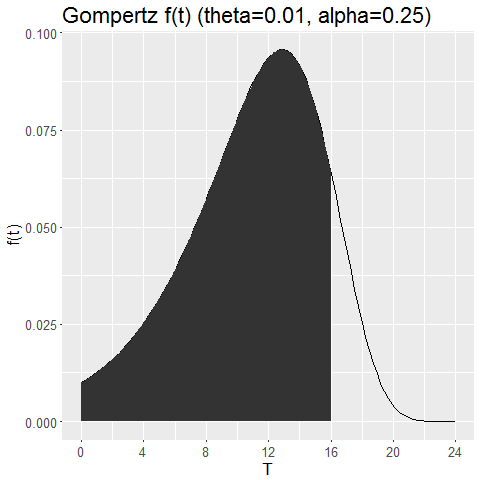
\includegraphics[width=0.98\textwidth]{Figures/shadedgompertzpdfL.png}\\
%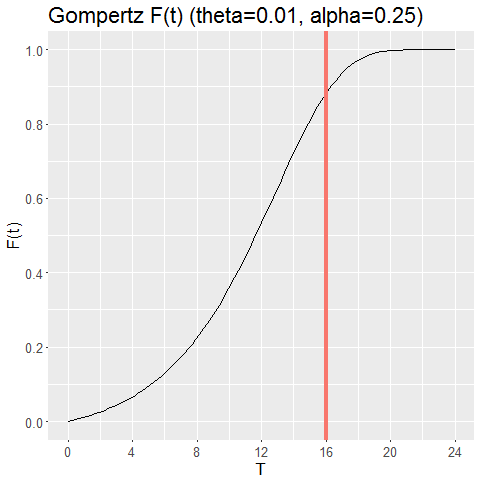
\includegraphics[width=0.98\textwidth]{Figures/gompertzcdfL12.png}
%\column{0.60\textwidth}
%\begin{clicker}{Which of the following applies to this picture?  The probability that an individual}
%\begin{enumerate}
%%\item will survive beyond time $t$.
%\item experiences the event at time $t$.
%\item experiences the event after time $t$.
%\item experiences the event before time $t$. %CORRECT  PR(T<t)
%\item does not experience the event before time $t$.
%\item does not experience the until event after time $t$.
%\end{enumerate}
%\end{clicker}
%\end{columns}
%\end{frame}
%
%\begin{frame}
%\begin{columns}
%\column{0.40\textwidth}
%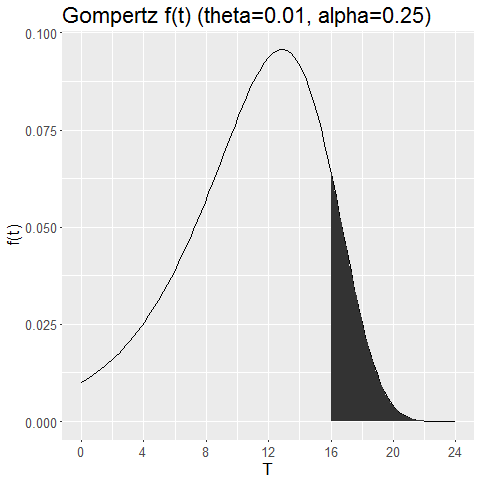
\includegraphics[width=0.98\textwidth]{Figures/shadedgompertzpdfU.png}\\
%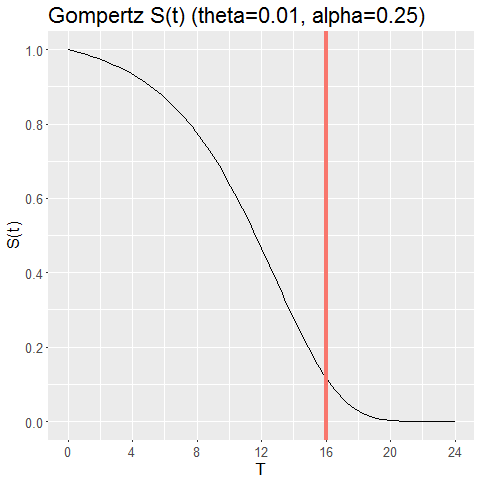
\includegraphics[width=0.98\textwidth]{Figures/gompertzsurvL12.png}
%\column{0.60\textwidth}
%\begin{clicker}{Which of the following applies to this picture?  The probability that an individual}
%\begin{enumerate}
%%\item will survive beyond time $t$. %CORRECT PR(T>t)
%\item experiences the event at time $t$.
%\item experiences the event after time $t$.
%\item experiences the event before time $t$.
%\item does not experience the event before time $t$.
%\item does not experience the event until after time $t$.  %CORRECT  PR(T>t)
%\end{enumerate}
%\end{clicker}
%\end{columns}
%\end{frame}

\begin{frame}
\frametitle{\grp}
\begin{clicker}{Suppose that the lifetime (in years) of a particular brand of light bulb, $T$, follows an exponential distribution with parameter $\lambda=5$.  The probability that a randomly selected light bulb lasts at least 7 years is given by...}
\begin{enumerate}
\item $F(7)$
\item $S(7)$ %correct
\item $F(5)$
\item $S(5)$
\end{enumerate}
\end{clicker}
\end{frame}

\begin{frame}
\frametitle{Example of survival function (exponential distribution)}
Suppose that the lifetime (in years) of a particular brand of light bulb, $T$, follows an exponential distribution with parameter $\lambda=5$.
\begin{enumerate}
\item Find the survival function $S(t)$.
\item[]
\item[]
\item Calculate the probability that a randomly selected light bulb lasts at least 7 years.
\item[]
\item[]
\item Calculate the proportion of light bulbs that last longer than 6 years.
\item[]
\item[]
\end{enumerate}
\end{frame}

\begin{frame}
\frametitle{}
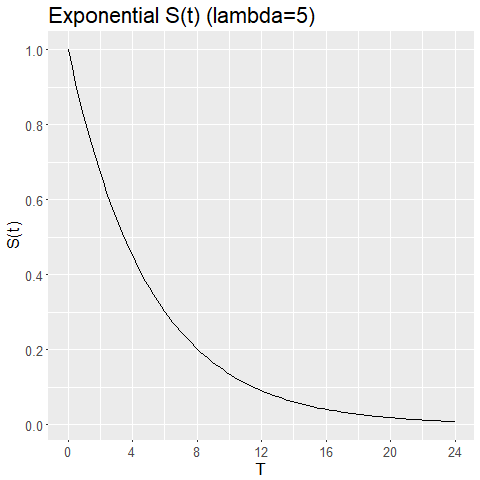
\includegraphics[width=0.70\textwidth]{Figures/expsurv.png}
\end{frame}

\begin{frame}
\frametitle{Example of survival function (Gompertz distribution)}
Recall the radiation exposure example. The time until death in months for mice exposed to a high dose of radiation follows a Gompertz distribution with parameters $\theta=.01$ and $\alpha = .25$.
\begin{enumerate}
\item Find the survival function $S(t)$.
\item[]
\item[]
\item Calculate the probability that a randomly chose mouse will live at least 18 months.
\item[]
\item[]
\item Calculate the probability that a randomly chosen mouse will die before 6 months.
\item[]
\item[]
\end{enumerate}
\end{frame}

\begin{frame}
\frametitle{}
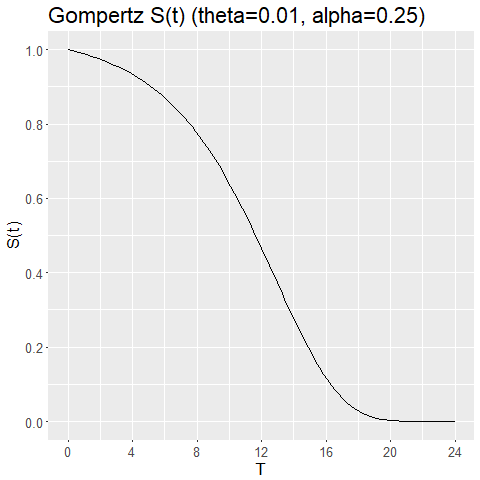
\includegraphics[width=0.70\textwidth]{Figures/gompertzsurv.png}
\end{frame}

\begin{frame}
\frametitle{Shape of survival function}
Suppose the survival curves correspond to the lifetimes of mice exposed to different doses of radiation; hence, the varying $\alpha$'s \\($T$ = time until death from radiation exposure). \\
\vskip3pt
\begin{columns}
\column{0.50\textwidth}
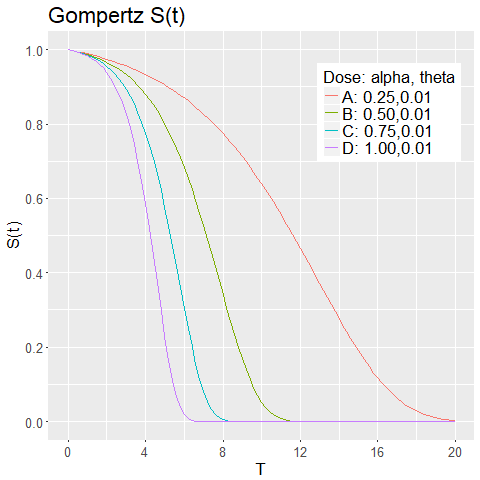
\includegraphics[width=0.98\textwidth]{Figures/gompertzsurv_varyalpha.png}
\column{0.50\textwidth}
\begin{clicker}{Which dose appear to be most lethal?}
\begin{enumerate}
\item Dose A
\item Dose B
\item Dose C
\item Dose D %correct
\end{enumerate}
\end{clicker}
\end{columns}
%Different probability distributions and/or different parameter values will result in different survival functions.
%Different shapes of survival curves indicate different patterns of event experience, i.e. survival, over time.
\end{frame}

\begin{frame}
\frametitle{Shape of survival function}
Recall the motorist reaction time data (seconds until a blocked driver honks the horn or flashes the high beams). Define $T=$ seconds until motorist reacts aggressively, and consider two possible probability models for $T$: Weibull($\lambda=5.74$, $\beta=1.6$) and exponential($\lambda=5.77$). \\
\vskip3pt
\begin{columns}
\column{0.50\textwidth}
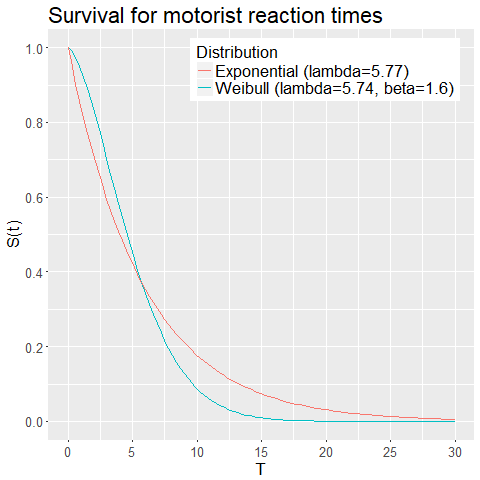
\includegraphics[width=0.98\textwidth]{Figures/motorist_surv_weib_exp.png}
\column{0.50\textwidth}
\begin{clicker}{Estimate the probability of survival for}
\bmp{.50\textwidth}
Weibull:\\
$S(10)$ = \\ %0.0879705
$S(20)$ = \\ %0.000630708
\emp
\bmp{.50\textwidth}
Exponential:\\
$S(10)$ = \\ %0.1767353
$S(20)$ = \\ %0.03123536
\emp
\end{clicker}
\end{columns}
\end{frame}


\begin{frame}
\frametitle{Comparing survival experiences}
Consider the data on the age when individuals took their first drink of alcohol - do the ``survival" experiences differ by gender?  Assume the probability model for males is Weibull($\lambda=18.28$, $\beta=2.64$) and for females is Weibull($\lambda=20.85$, $\beta=2.52$).
\vskip3pt
\begin{columns}
\column{0.50\textwidth}
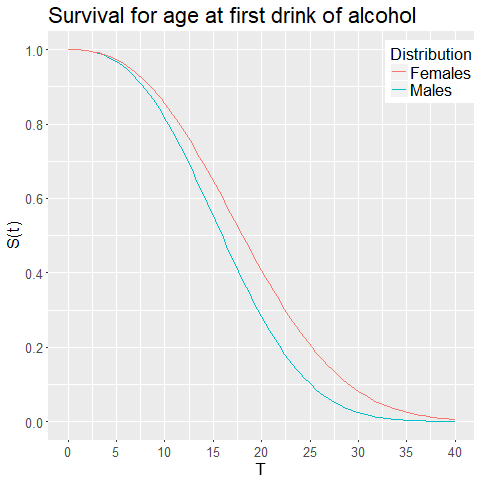
\includegraphics[width=0.98\textwidth]{Figures/drink_surv_weib.png}
\column{0.50\textwidth}
\begin{enumerate}
\item Compare the survival experiences of males and females.
\item[] %males experience their first drink of alcohol before females
\item[] %survival prob for females always larger than survival prob for males, regardless of age
\item Estimate $S(20)$
\item[] Males: %0.281408 (alcohol free after age 20)
\item[] Females:  %0.4063963 (alcohol free after age 20)
\end{enumerate}
\end{columns}
\end{frame}

%===========================================================================================================================
\section[Hazard function]{Hazard function}
%===========================================================================================================================
\subsection{}
\begin{frame}
\tableofcontents[currentsection, hideallsubsections]
\end{frame}

\begin{frame}
\frametitle{Motorist reaction time example}
Let $T$ (time until motorist reacts aggressively) follow a Weibull distribution with parameters $\lambda=5.74$ and $\beta=1.6$.  The survival function is given by
\begin{eqnarray}
S(t)=\exp\left[ -\left(\frac{t}{5.74} \right)^{1.6} \right] \nonumber
\end{eqnarray}
What is the chance that a motorist blocked behind a vehicle does not act aggressively for at least 2 seconds?
\vskip100pt
%\item Suppose that a motorist has been waiting for two seconds behind a stopped vehicle. What is the chance that the motorist will react aggressively within the next 1 second?
\end{frame}

\begin{frame}
\frametitle{Motorist reaction time example, continued}
Let $T$ (time until motorist reacts aggressively) follow a Weibull distribution with parameters $\lambda=5.74$ and $\beta=1.6$.  The survival function is given by
\begin{eqnarray}
S(t)=\exp\left[ -\left(\frac{t}{5.74} \right)^{1.6} \right] \nonumber
\end{eqnarray}
Suppose that a motorist has been waiting for two seconds behind a stopped vehicle. What is the chance that the motorist will react aggressively within the next 1 second?
\vskip100pt
\end{frame}

\begin{frame}
\frametitle{Motorist reaction time example, continued}
\end{frame}

\begin{frame}
\frametitle{Motorist reaction time example, summary}
\begin{itemize}
\item The survival function is useful for examining the probability that a randomly selected individual survives beyond time $t$.
\item[] %We assessed the unconditional probability of survival
\item[]
\item[]
\item The survival function does not assess what will happen to an individual immediately beyond time $t$ \textit{conditional} on surviving to time $t$.
\item[] %We assessed the conditional probability of experiencing the event in the next "fraction" of time given survival to a particular time
\item[]
\item[]
\end{itemize}
\end{frame}

\begin{frame}
\frametitle{Hazard function}
\begin{itemize}
\item Viewed in a slightly different way, we are attempting to assess the \textit{risk} or \textit{potential} that an individual who has not done so already, will experience the event of interest in the next instant (or ``very small") amount of time.
\item[]
\item This (conditional) \textit{risk} is the basis for the concept called \textbf{hazard} and for the function that describes changes in hazard over time called the \textbf{hazard function}.
\item[]
\item If we are trying to assess the risk in the next ``instant" of time, given that the target event has yet to occur, then let's try to develop this idea using conditional probability...
\item[]
\end{itemize}
\end{frame}

\begin{frame}
\frametitle{Motorist reaction time: assessing risk}
Now let's see what happens when the subsequent interval of time decreases from 1 second to 1/2 second, and then to 1/4 of a second:
\begin{enumerate}
\item If a motorist has been blocked for at least 2 seconds, then find the probability that the motorist will react aggressively within the next half second. Compare your answer to the conditional probability found in part (2) of the previous example above.

\item Repeat (1) for the next quarter second.

\item What appears to be happening as the amount of elapsed time after 2 seconds becomes very {small}?

\item Now generalize: If a motorist has not reacted aggressively for at least $t$ seconds, then as the next interval of time shrinks to 0 seconds, what is the chance that a motorist reacts aggressively in that interval?
%Let \Delta t = small elapsed amount of time
\end{enumerate}
\end{frame}

\begin{frame}
\frametitle{Motorist reaction time: assessing risk, cont.}
\end{frame}

\begin{frame}
\frametitle{Motorist reaction time: assessing risk, cont.}
\end{frame}

\begin{frame}
\frametitle{Hazard function}
\begin{itemize}
\item So we cannot assess instantaneous risk of event occurrence at time $t$ using conditional probability, since it will always approach 0 as $\Delta t$ approaches 0.

\item But if we scale the limiting conditional probability by dividing by the change in time, $\Delta t$, then we get the following \textit{instantaneous rate}, known as the \textbf{hazard function}, denoted $h(t)$:
\end{itemize}
\vskip100pt
\end{frame}

\begin{frame}
\frametitle{Hazard function}
\begin{itemize}
\item  The hazard function $h(t)$ describes the rate of ``failure" or ``event experience" \textit{per unit of time} in an instant after time $t$ (sometimes called the \textit{instantaneous rate of failure}), \textit{conditional} on surviving to time $t$.
\item For \textit{continuous} $T$, $h(t)$ is \textit{not} a probability and should never be interpreted as such. The only restriction on values of $h(t)$ is that $h(t) \geq 0$.
\item In other fields, $h(t)$ is known as:
\begin{itemize}
\item Conditional failure rate (reliability theory).
\item Force of mortality (demography).
\item Intensity function (stochastic processes).
\item Age-specific failure rate (epidemiology).
\end{itemize}
\end{itemize}
General connection between the hazard function $h(t)$ and the survival function $S(t)$:
\vskip30pt
\end{frame}

\begin{frame}
\frametitle{Formal definition of $h(t)$}
\begin{itemize}
\item The formal definition for the hazard function $h(t)$ is:
\item[]
\begin{eqnarray}
h(t)= \lim_{\Delta t\rightarrow 0}\frac{P(t<T\leq t+\Delta t|T \geq t)}{\Delta t} \nonumber
\end{eqnarray}
\item[]
\item[]
where $\Delta t$ represents a \textit{small} elapsed amount of time.
\item[]
\item From this definition, we can derive another useful mathematical expression for $h(t)$:
\end{itemize}
\vskip100pt
\end{frame}

\begin{frame}
\frametitle{Motorist reaction time: Weibull hazard function}
Suppose that the time until the motorist reacts aggressively follows a Weibull probability model with parameters $\beta=1.6$ and $\lambda=5.74$.  Note that:
\begin{eqnarray}
f(t) = \frac{1.6t^{.6}}{(5.74)^{1.6}}\exp \left[-\left(\frac{t}{5.74}\right)^{1.6} \right] \nonumber
\end{eqnarray}
\vskip5pt
\begin{eqnarray}
S(t)=\exp\left[ -\left(\frac{t}{5.74} \right)^{1.6} \right] \nonumber
\end{eqnarray}
\end{frame}

\begin{frame}
\frametitle{Motorist reaction time: Weibull hazard function}
\begin{enumerate}
\item Derive the hazard function using the expression $h(t)=\frac{f(t)}{S(t)}$
%\item Derive the hazard function using the expression $h(t)=-\frac{d}{dt}\ln[S(t)]$
%\item The hazard and survival functions (curves) are displayed on \textbf{Slide 84}. Examine the plots and comment on aggressive behavior over time.
\end{enumerate}
\vskip150pt
\end{frame}

\begin{frame}
\frametitle{Motorist reaction time: Weibull hazard function}
\begin{enumerate}
\setcounter{enumi}{1}
%\item Derive the hazard function using the expression $h(t)=\frac{f(t)}{S(t)}$
\item Derive the hazard function using the expression $h(t)=-\frac{d}{dt}\ln[S(t)]$
%\item The hazard and survival functions (curves) are displayed on \textbf{Slide 84}. Examine the plots and comment on aggressive behavior over time.
\end{enumerate}
\vskip150pt
\end{frame}

\begin{frame}
\frametitle{Motorist reaction time: Weibull hazard function}
\begin{columns}
\column{0.5\textwidth}
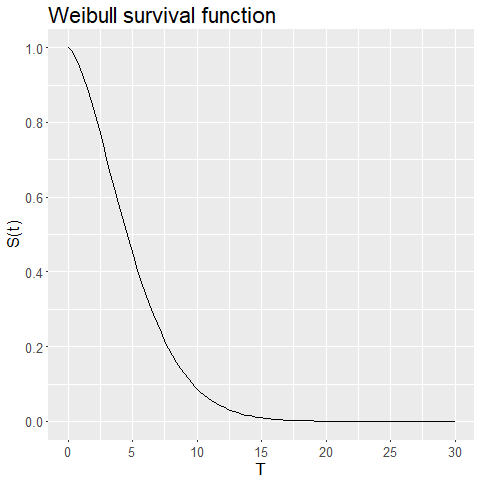
\includegraphics[width=0.98\textwidth]{Figures/motorist_surv_weib.png}
\column{0.5\textwidth}
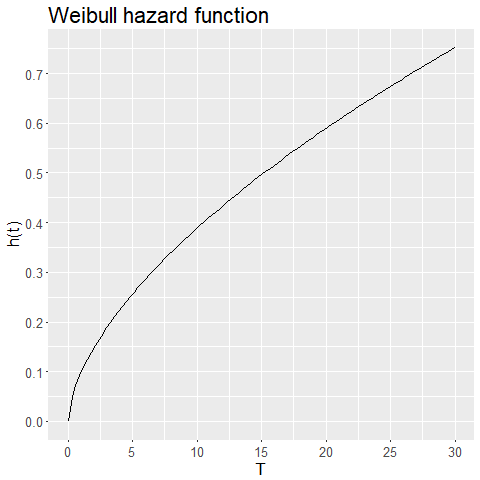
\includegraphics[width=0.98\textwidth]{Figures/motorist_haz_weib.png}
\end{columns}
\end{frame}

\begin{frame}
\frametitle{Motorist reaction time: Weibull hazard function}
\begin{enumerate}
\setcounter{enumi}{2}
%\item Derive the hazard function using the expression $h(t)=\frac{f(t)}{S(t)}$
%\item Derive the hazard function using the expression $h(t)=-\frac{d}{dt}\ln[S(t)]$
\item Examine the survival and hazard plots and comment on aggressive behavior over time.
\end{enumerate}
\vskip150pt
%1 - survival goes up, hazard goes down
%2 - hazard curve: is always increasing (doesn't have to be the case)
%3 - hazard curve: for those not reacting aggressively until time t, the instantaneous rate of reacting aggressively always increases
%4 - increase between 0 and 2 is faster than increase at later time points -> hazard increases really fast in first couple of seconds
\end{frame}

\begin{frame}
\frametitle{Motorist reaction time: exponential hazard function}
Assume that the time until a motorist acts aggressively follows an exponential distribution with $\lambda=5.77$.
\begin{enumerate}
\item Find the hazard function $h(t)$.
\end{enumerate}
\vskip150pt
\end{frame}

\begin{frame}
\frametitle{Motorist reaction time: exponential hazard function}
\begin{columns}
\column{0.5\textwidth}
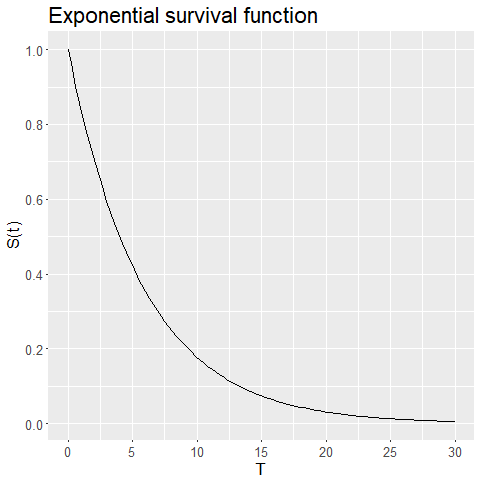
\includegraphics[width=0.98\textwidth]{Figures/motorist_surv_exp.png}
\column{0.5\textwidth}
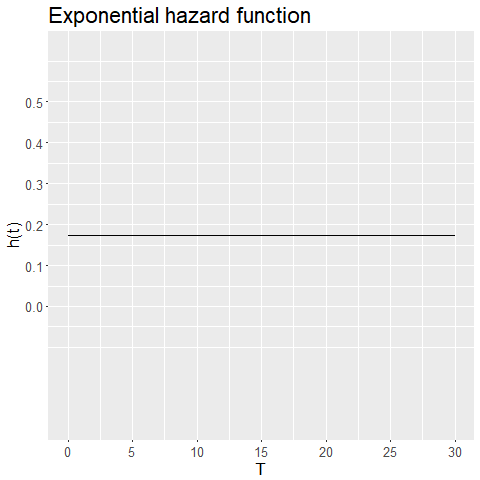
\includegraphics[width=0.98\textwidth]{Figures/motorist_haz_exp.png}
\end{columns}
\end{frame}

\begin{frame}
\frametitle{Motorist reaction time: exponential hazard function, cont.}
\begin{enumerate}
\setcounter{enumi}{1}
\item What does this result imply about the risk of a randomly selected motorist acting aggressively?
%hazard function is constant (doesn't depend on time, applies for all exponentials)
%not a very likely situation, but has an easy interpretation
%for 1000 individuals who havent reacted aggressively by 2 seconds, 173 will react aggressively in the next second
%can use time here, but not in other h(t)
\end{enumerate}
\vskip150pt
\end{frame}

\begin{frame}
\frametitle{Age at first drink: logistic hazard function}
Another probability model used for describing time-to-event random variables is the \textbf{logistic distribution} with parameters $\alpha$ and $\beta$, which has probability density function given by:
\vskip3pt
\begin{eqnarray}
f(t) = \frac{\exp^{-(t-\alpha)/\beta}} {\beta \left[1 + \exp^{-(t-\alpha)/\beta} \right]^2} ,~\beta > 0 \nonumber
\end{eqnarray}
\vskip3pt
Recall data on the age of first drink of alcohol, and suppose that $T=$ ``age at first drink of alcohol" follows the {logistic distribution} with parameter values $\alpha=16.74$ and $\beta=2.8$.
\end{frame}

\begin{frame}
\frametitle{Age at first drink: logistic hazard function}
\begin{columns}
\column{0.5\textwidth}
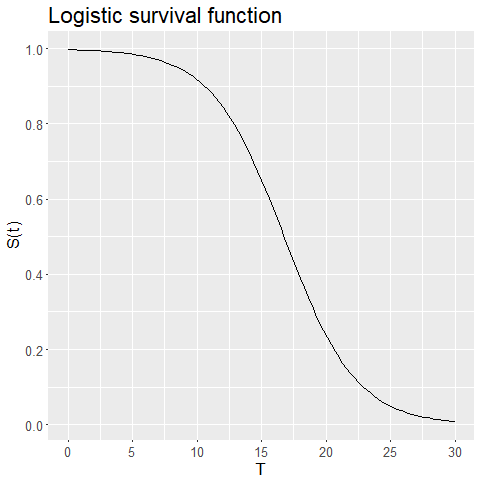
\includegraphics[width=0.98\textwidth]{Figures/drink_surv_log.png}
\column{0.5\textwidth}
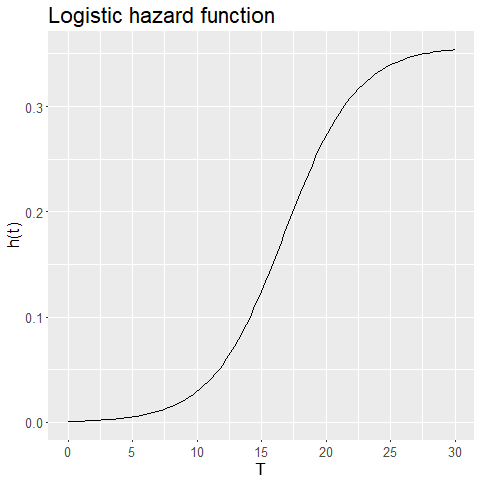
\includegraphics[width=0.98\textwidth]{Figures/drink_haz_log.png}
\end{columns}
\end{frame}

\begin{frame}
\frametitle{Age at first drink: logistic hazard function}
Comment on how the risk of first alcoholic drink changes with age.
\vskip150pt
%0-12 years risk of frist drink increases slowly
%13-26 years risk increases rapidly
%>26 years risk increases slowly
%risk always increases, but rate of risk changes
\end{frame}

%===========================================================================================================================
\section[Cumulative hazard function]{Cumulative hazard function}
%===========================================================================================================================
\subsection{}
\begin{frame}
\tableofcontents[currentsection, hideallsubsections]
\end{frame}

\begin{frame}
\frametitle{Cumulative hazard function}
\begin{itemize}
\item Sometimes the changes in $h(t)$ are subtle, and it can be difficult to describe periods of increasing and decreasing risk. %(this will become very apparent when we examine the \textit{estimated} hazard function later).

\item An alternative method to assess and describe how the hazard rates change over time is to
investigate the accumulation of the hazard rates over time, and look for patterns in
the \textbf{cumulative hazard}.

\item The function that allows us to examine accumulated hazard over time is called the \textbf{cumulative hazard function}.

\item The cumulative hazard function, denoted $H(t)$, is the accumulated
risk (hazard) of experiencing an event up to time $t$, and is given
by:
%\begin{eqnarray}
%H(t)= \mbox{the accumulation of the hazard rate $h(t)$ for time $T$ between 0 and $t$} \nonumber
%\end{eqnarray}
%or mathematically:
%\begin{eqnarray}
%\boxed{H(t)=\int_0^th(u)du} \nonumber
%\end{eqnarray}
%\item In general, $H(t)$ increases as $t$ increases %($H(t)$ is constant only when $h(t)=0$)
%\item \textbf{Note}: $H(t)$ is neither a rate nor a probability
\end{itemize}
\vskip50pt
\end{frame}

\begin{frame}
\frametitle{Cumulative hazard function, cont.}
\begin{itemize}

%\item The benefits of using the cumulative hazard function to describe time-to-event data will become more clear when we discuss an estimator of the hazard function.

%\item It turns out that estimators of $h(t)$ based on sample data are extremely rough and erratic, and are not very useful.  An estimator of $H(t)$ can provide better information about the risk of event experience than estimators of $h(t)$ can.

\item An important point is that the cumulative hazard function $H(t)$ is neither a probability, nor a rate -
it is simply an accumulation of (hazard) rates over time.

\item Since $H(t)$ is \textit{accumulating} rates over time, it never decreases (and rarely ever remains constant).

\item Therefore, we can examine the nature of the increase in $H(t)$ (perhaps over specific time intervals of interest), i.e. whether the \textit{rate} of increase in the curve is increasing or decreasing.

\item How do we measure the rate of increase in $H(t)$ at a particular point in time?
%Slope of the curve at a particular time
\vskip .8in
\end{itemize}
\end{frame}

\begin{frame}
\frametitle{Age at first drink: cumulative hazard function}
\begin{columns}
\column{0.5\textwidth}
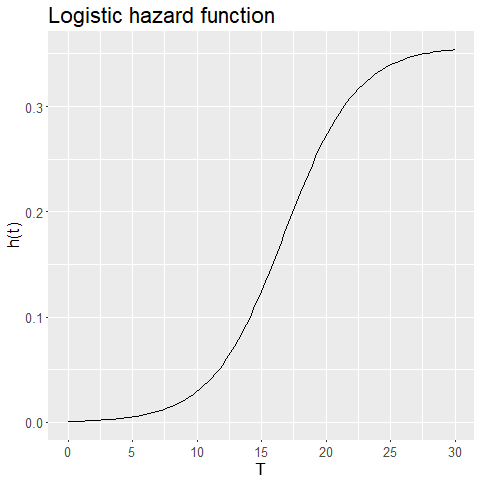
\includegraphics[width=0.98\textwidth]{Figures/drink_haz_log.png}
\column{0.5\textwidth}
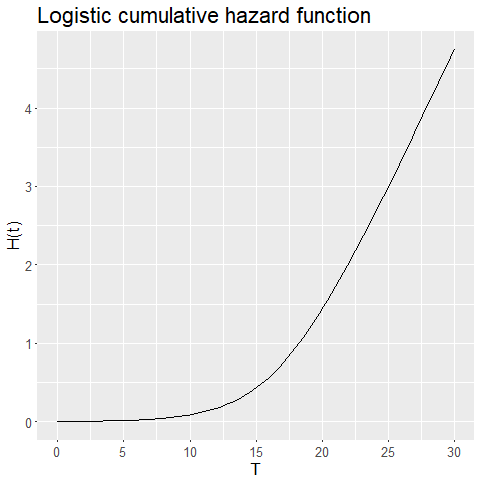
\includegraphics[width=0.98\textwidth]{Figures/drink_cum_haz_log.png}
\end{columns}
\end{frame}

%\begin{frame}
%\frametitle{Relationship between $H(t)$ and $h(t)$}
%%The change in the \textit{rate of increase} in $H(t)$ over time can be examined to understand how $h(t)$ changes over time.
%%Examine the relationship between the {rate} of increase in $H(t)$ (bottom plots) and the values of $h(t)$ (top plots) over time:
%
%\end{frame}


\begin{frame}
\frametitle{Relationship between $H(t)$ and $h(t)$, cont.}
\begin{itemize}
%\item By examining the cumulative hazard function, we will be able to detect when the hazard is increasing,
%decreasing, or remaining relatively constant.
\item Period of time when the \textit{rate} of increase in $H(t)$ is \textit{increasing} indicates that:
% then $h(t)$ is increasing (over the same interval of time).
\item[]
\item[]
\item Period of time when the \textit{rate} of increase in $H(t)$ is \textit{decreasing} indicates that:
%$h(t)$ is decreasing.
\item[]
\item[]
\item Period of time when the \textit{rate} of increase in $H(t)$ is \textit{constant} indicates that:
% $h(t)$ is constant (and greater than zero).
\item[]
\item[]
\item Period of time when the \textit{rate} of increase in $H(t)$ is 0 indicates that:
%$h(t)$ is 0.
\item[]
\item[]
\end{itemize}
\end{frame}

\begin{frame}
\frametitle{Expressions for $H(t)$}
Recall that the $H(t)$ is given by:
\begin{eqnarray}
H(t)=\int_0^th(y)dy \nonumber
\end{eqnarray}
\vskip20pt
It can also be shown that:
\begin{eqnarray}
H(t)= -\ln[S(t)] \nonumber
\end{eqnarray}
\end{frame}

\begin{frame}
\frametitle{Motorist reaction time: exponential cumulative hazard}
Consider an exponential($\lambda=5.77$) probability model for the motorist reaction time variable.  Derive $H(t)$.
\begin{eqnarray}
h(t)= \frac{1}{5.77} \nonumber
\end{eqnarray}
\vskip200pt
\end{frame}

\begin{frame}
\frametitle{Motorist reaction time: exponential $h(t)$ and $H(t)$}
\begin{columns}
\column{0.5\textwidth}
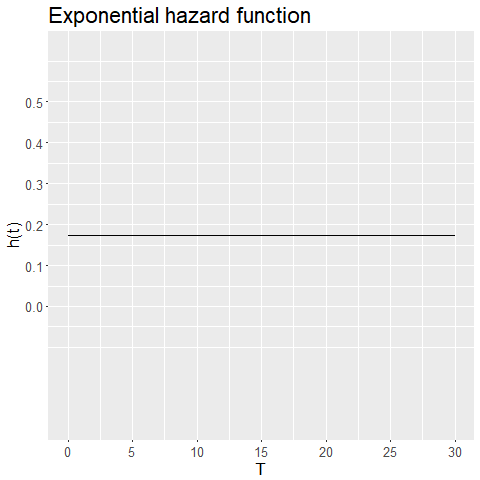
\includegraphics[width=0.98\textwidth]{Figures/motorist_haz_exp.png}
\column{0.5\textwidth}
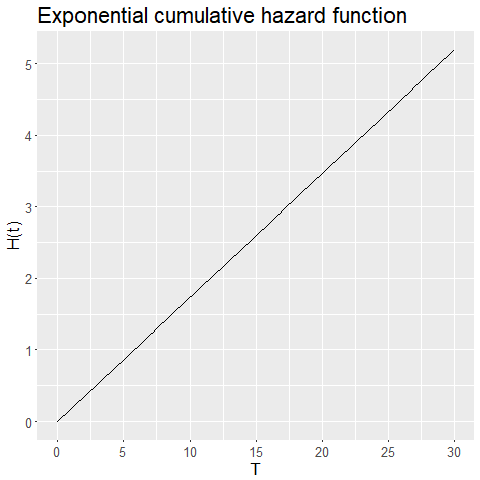
\includegraphics[width=0.98\textwidth]{Figures/motorist_cum_haz_exp.png}
\end{columns}
%hazard remains constant, cumulative hazard is increasing at constant rate
\end{frame}

\begin{frame}
\frametitle{Motorist reaction time: Weibull cumulative hazard}
Consider a Weibull($\beta=1.6$ and $\lambda=5.74$) probability model for the motorist reaction time variable.  Derive $H(t)$.
\begin{eqnarray}
S(t)=\exp\left[ -\left(\frac{t}{5.74} \right)^{1.6} \right] \nonumber
\end{eqnarray}
\vskip200pt
\end{frame}

\begin{frame}
\frametitle{Motorist reaction time: Weibull $h(t)$ and $H(t)$}
\begin{columns}
\column{0.5\textwidth}
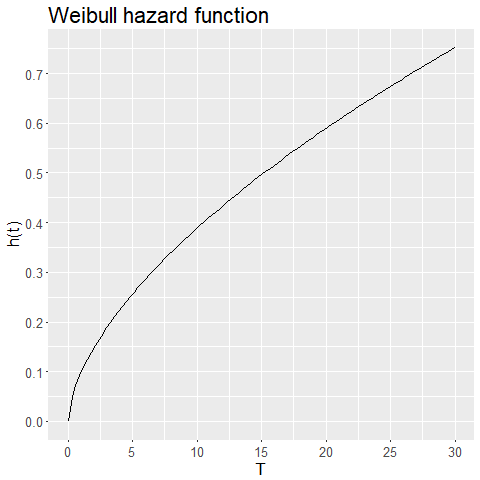
\includegraphics[width=0.98\textwidth]{Figures/motorist_haz_weib.png}
\column{0.5\textwidth}
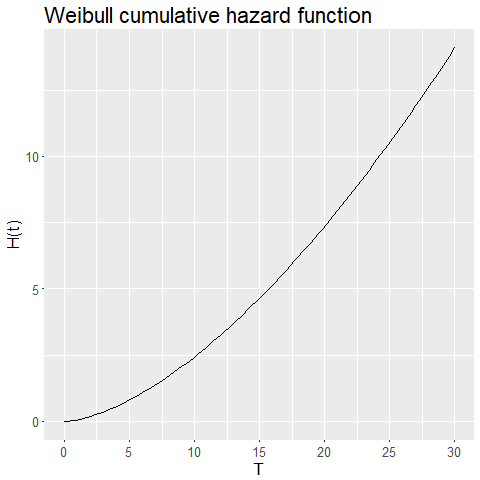
\includegraphics[width=0.98\textwidth]{Figures/motorist_cum_haz_weib.png}
\end{columns}
\end{frame}


%===========================================================================================================================
\section[Summary]{Summary}
%===========================================================================================================================
\subsection{}
\begin{frame}
\tableofcontents[currentsection, hideallsubsections]
\end{frame}

\begin{frame}
\frametitle{Probability models for $T$}
\begin{tabular}{ll}
Exponential & $f(t)=\frac{1}{\lambda} \exp(-t/\lambda)$ \\
[1ex] \\
Weibull & $f(t)=\frac{\beta t^{\beta-1}}{\lambda^{\beta}}\exp(-(t/\lambda)^\beta)$ \\
[1ex] \\
Gompertz & $f(t)=\theta e^{\alpha t}\exp\left[\frac{\theta}{\alpha}\left(1-e^{\alpha t}\right)  \right]$ \\
[1ex] \\
Lognormal & $f(t)=\frac{\exp\left[ -\frac{1}{2}\left(\frac{\ln(t)-\mu}{\sigma} \right)^2 \right]}{t(2\pi)^{1/2}\sigma}$ \\
[1ex] \\
Logistic & $f(t) = \frac{\exp^{-(t-\alpha)/\beta}} {\beta \left[1 + \exp^{-(t-\alpha)/\beta} \right]^2}$ \\
\end{tabular}
\end{frame}

\begin{frame}
\frametitle{Relationships between functions of $T$}
{\renewcommand{\arraystretch}{1.8}
\begin{tabular}{ll}
\hline
Function & Relationships  \\
\hline
PDF & ${f(t)=\frac{d}{dt}F(t)}$\\
CDF  & ${F(t)=\int_0^t f(y)dy}$\\
Survival & ${S(t)=1-F(t)=\exp[-H(t)]=\exp[-\int_0^th(y)dy]}$ \\
Hazard & ${h(t)=f(t)/S(t)=-\frac{d}{dt}\ln[S(t)]}$ \\
Cum. Haz. & ${H(t)=\int_0^t h(y)dy=-\ln[S(t)]}$\\
\hline
\end{tabular}}
\end{frame}

\end{document} 